%%%
 %
 % Copyright (C) 2019 Ángel Iván Gladín García
 %
 % This program is free software: you can redistribute it and/or modify
 % it under the terms of the GNU General Public License as published by
 % the Free Software Foundation, either version 3 of the License, or
 % (at your option) any later version.
 %
 % This program is distributed in the hope that it will be useful,
 % but WITHOUT ANY WARRANTY; without even the implied warranty of
 % MERCHANTABILITY or FITNESS FOR A PARTICULAR PURPOSE.  See the
 % GNU General Public License for more details.
 %
 % You should have received a copy of the GNU General Public License
 % along with this program.  If not, see <http://www.gnu.org/licenses/>.
%%%

%%%%%%%%%%%%%%%%%%%%%%%%%%%%%%%%%%%%%%%%%%%%%%%%%%%%%%%%%%%%%%%%%%%%%%%%%%%%%%%%%%%%%%%%%
\documentclass[11pt,letterpaper]{article}
\usepackage[utf8]{inputenc}
\usepackage[spanish]{babel}
\usepackage[margin=1in]{geometry}
 
\usepackage{listings}
\usepackage{color}
\usepackage{graphicx}
\usepackage{enumerate}
\usepackage{enumitem}

\usepackage{longtable}
\usepackage{hyperref}
\usepackage{commath}

\usepackage{minted}
\usemintedstyle{emacs}

\usepackage{bbm}
\usepackage{dsfont}
\usepackage{mathrsfs}
\usepackage{amsmath,amsthm,amssymb}
\usepackage{mathtools}
\usepackage{longtable}
%%%%%%%%%%%%%%%%%%%%%%%%%%%%%%%%%%%%%%%%%%%%%%%%%%%%%%%%%%%%%%%%%%%%%%%%%%%%%%%%%%%%%%%%%%%%%%%%5

\usepackage{import}

\usepackage[utf8]{inputenc}
 
\usepackage{listings}
\usepackage{color}
 
\definecolor{codegreen}{rgb}{0,0.6,0}
\definecolor{codegray}{rgb}{0.5,0.5,0.5}
\definecolor{codepurple}{rgb}{0.58,0,0.82}
\definecolor{backcolour}{rgb}{0.95,0.95,0.92}
 
\lstdefinestyle{mystyle}{
    backgroundcolor=\color{backcolour},   
    commentstyle=\color{codegreen},
    keywordstyle=\color{magenta},
    numberstyle=\tiny\color{codegray},
    stringstyle=\color{codepurple},
    basicstyle=\footnotesize,
    breakatwhitespace=false,         
    breaklines=true,                 
    captionpos=b,                    
    keepspaces=true,                 
    numbers=left,                    
    numbersep=5pt,                  
    showspaces=false,                
    showstringspaces=false,
    showtabs=false,                  
    tabsize=2
}
 
\lstset{style=mystyle}
%%%%%%%%%%%%%%%%%%%%%%%%%%%%%%%%%%%%%%%%%%%%%%%%%%%%%%%%%%%%%%%%%%%%%%%%%%%%%%%%%%%%%%%%%


%%%%%%%%%%%%%%%%%%%%%%%%%%%%%%%%%%%%%%%%%%%%%%%%%%%%%%%%%%%%%%%%%%%%%%%%%%%%%%%%%%%%%%%%%
\newcommand{\Z}{\mathbb{Z}}
\newcommand{\N}{\mathbb{N}}
\newcommand{\Q}{\mathbb{Q}}
\newcommand{\R}{\mathbb{R}}
\newcommand{\Oh}{\mathcal{O}} %% Notacion "O"
\newcommand{\ent}{\Longrightarrow}
\newcommand{\lra}{\longrightarrow}
\newcommand{\ra}{\rightarrow}
\newcommand{\sii}{\Longleftrightarrow}
\newcommand{\clase}[1]{\overline{#1}}  %% barrita sobre letras
\newcommand{\ord}{\text{ord}}
\newcommand{\leg}[2]{\left( \frac{#1}{#2}\right)} %% Simbolo de Legendre
\newcommand{\sol}{\textbf{\underline{Solución}: }} %% Solución

%%%%%%%%%%%%%%%%%%%%%%%%%%%%%%%%%%%%%%%%%%%%%%%%%%%%%%%%%%%%%%%%%%%%%%%%%%%%%%%%%%%%%%%%%

\begin{document}

%%%%%%%%%%%%%%%%%%%%%%%%%%%%%%%%%%%%%%%%%%%%%%%%%%%%%%%%%%%%%%%%%%%%%%%%%%%%%%%%%%%%%%%%%
\title{
    \vspace{-2cm}
        Universidad Nacional Autónoma de México\\
        Facultad de Ciencias\\
        Criptografía y Seguridad\\
    \vspace{.5cm}
    \large
        \textbf{Tarea 3}\\
        \textbf{Curvas elípticas}
}
\author{
    Ángel Iván Gladín García\\
    No. cuenta: 313112470\\
    \texttt{angelgladin@ciencias.unam.mx}
    \and
    Melanie Bautista Cruz\\
    No. cuenta: 313181711\\
    \texttt{mbautista@ciencias.unam.mx}
}
\date{24 de Mayo 2019}
\maketitle
%%%%%%%%%%%%%%%%%%%%%%%%%%%%%%%%%%%%%%%%%%%%%%%%%%%%%%%%%%%%%%%%%%%%%%%%%%%%%%%%%%%%%%%%%

%%%%%%%%%%%%%%%%%%%%%%%%%%%%%%%%%%%%%%%%%%%%%%%%%%%%%%%%%%%%%%%%%%%%%%%%%%%%%%%%%%%%%%%%%
\newtheorem{theorem}{Teorema}
\newtheorem{example}{Ejemplo}
\newtheorem{corollary}{Corolario}
\newtheorem{lemma}{Lemma}
\newtheorem{definition}{Definición}
\newtheorem{prop}{Proposición}
%%%%%%%%%%%%%%%%%%%%%%%%%%%%%%%%%%%%%%%%%%%%%%%%%%%%%%%%%%%%%%%%%%%%%%%%%%%%%%%%%%%%%%%%%


%%%%%%%%%%%%%%%%%%%%%%%%%%%%%%%%%%%%%%%%%%%%%%%%%%%%%%%%%%%%%%%%%%%%%%%%%%%%%%%%%%%%%%%%%

%%%%%%%%
\section{Sea la curva elíptica $E := 0 = y^2 - x^3 - x - 9$ definida sobre $\Z_{17}$}

\begin{figure}[H]
\centering
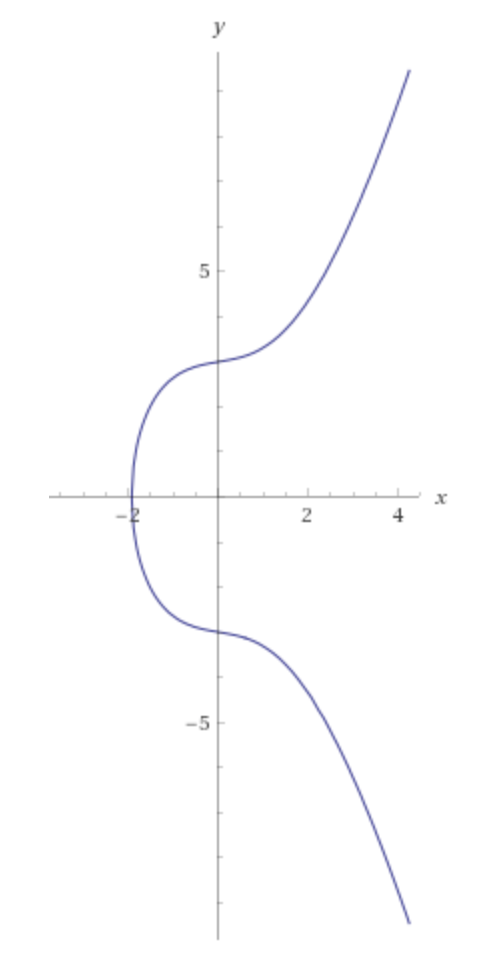
\includegraphics[width=0.2\textwidth]{assets/curva.png}
\caption{Curva elíptica de la forma $y^2 = x^3 + x + 9$}
\end{figure}

\begin{enumerate}[label=(\roman*)]
    \item Calcule y muestre todos los puntos de $E$.\\
    \sol Por definición se consideran los puntos con coordenadas en algún campo $L \supseteq K$ que se
    escribirá como $E(L)$, por definición, este conjunto siempre contiene al punto $\infty$.
    $$E(L) = \{\infty\} \cup \{(x,y) \in L \times L \mid y^2 = x^3 + Ax + B\}$$
    Para encontrar los puntos de $E$, se procederá por calcular todos los puntos en la curva
    dejando correr los valores de $x \in [0,16]$ y resolver para $y$. Sutituyendo cada uno de esos
    puntos y encontrar el valor $y$ que resuelva la ecuación. Para hacerlo se hizo
    un programa en \textit{Python}.
    
    \inputminted{python}{assets/encontrar_puntos.py}
    
    Con el programa previo se puede concluir que $|E| = 25$ y que los puntos son:
    $$\{ \Oh \} \cup \{(0, 3), (0, 14), (2, 6), (2, 11), (4, 3), (4, 14), (7, 6), (7, 11), (8, 6),$$
    $$(8, 11), (9, 4), (9, 13), (10, 4), (10, 13), (11, 5), (11, 12), (12, 7), (12, 10), (13, 3),$$
    $$(13, 14), (14, 8), (14, 9), (15, 4), (15, 13)\}$$

    \item Alicia desea enviar el siguiente mensaje $C = (a, b) = ((12, 7), (11, 12))$ a Bob,
    los parámetros públicos de Bob son $\alpha = (0, 3) \in E$ una raíz primitiva y 
    $\beta = (13, 3)$, donde $\beta = s \alpha$ y $s$ su llave privada. Usa cualquier algoritmo
    mencionado en la sección 5.2 del libro \textbf{Elliptic Curves Number Theory and Cryptography de Lawrence C. Washington}
    Para resolver el PLD.\\
    \sol Se uso estos scripts\footnote{\url{https://github.com/ashutosh1206/Crypton/tree/master/Elliptic-Curves} 
    para la manipulación y operaciones sobre curvas elípticas.}. Siguiendo el
    algoritmo\footnote{Página 146}, $\alpha$ la raíz primitiva existe
    una $k$ la que $M_1 = k\alpha$ que esto es $M_1 = (12,7) = k(0,3)$ teniendo que essto el la primera entrada
    de $C$. Para encontrar la $k$ de $M_2$ (que es la segunda entrada de $C$) que es
    $(11,12) = M_2 = M + kB = M + k(13,3)$.\\
    Tomando $m \geq \sqrt{5}$ calculando $n(0,3)$ con $n \in [0, 4]$. Encontrando los inversos en 
    $\Z_{17}^{*}$ y como $0(0,3) = (0,3) - (0,3) 0$, $1(0,3) = (0,3)$ y $2(0,3) = (0,3) + (0,3)$.\\
    Entonces $3(0,3) = (0,3) + (9,4)$. con $k = 3$ y $3(0,3) = (12,7)$.\\
    Calculando $kB = k(13,3)$ entonces $kB = 3B = (7,11)$, entonces $M=(11,12)-(7,11)$ quedando así
    $M=(14,9)$.
    
    \item A partir de la información encontrada en $(ii)$ descifra el mensaje enviado a Bob.\\
    \sol Usando ElGamal\footnote{Página 175} siguiendo la fórmula de:
    $$M = M_2 - sM_1$$
    Se tiene que $M = (11,12) - s(12,7) = (11,12) - 7(12,7) = (11,2) - (7,11) = (11,12) + (7,6) = (14,9)$.
    Donde el mensaje original es $M = (14,9)$.

\end{enumerate}
%%%%%%%%

%%%%%%%%
\section{Sea $E := y^2 + 20x = x^3 +21 \mod{35}$ y sea $P = (15, -4) \in E$.}

\begin{enumerate}[label=(\roman*)]
    \item Factoriza 35 tratando de calcular $3P$.\\
    \sol Sea $E$ la curva elíptica $y^2 = x^3 - 20x + 21 \mod{35}$ y sea $P = (15, -4)$.
    Primero se procedera a calcular la línea tangente pendiente del punto $P$. Dado que solo se tiene
    un punto, se usará la siguiente fórmula\footnote{Se explica bien el porqué en la página 13 de
    la bibliografía.}:
    $$m = \frac{dy}{dx} = \frac{3x_1^2 + A}{2y_1}$$
    
    Entonces para encontrar $m$ del punto $P$ se aplicará la fórmula previa
    $$m = \frac{3x_1^2 + A}{2y_1} = \frac{3(15)^2 - (20)}{2(-4)} = -\frac{25}{8} \mod{35}$$
    
    Se obtendrá el máximo común divisor del denominador de $m$ y el módulo $p$,  $gcd(8, 35) = 1$. Dado que
    es 1, se calculará\footnote{Use esta herrmienta para calcular inversos multiplicativos módulo $p$,
    \url{https://planetcalc.com/3311/}}
    el inverso módulo $p$ del denominador de la pendiente $m$, el cual es, $8^{-1} \equiv 22 \mod 35$.\\
    Teniendo el inverso, la pendiente queda como:
    $$-\frac{25}{8} \cdot (8^{-1}) = -\frac{25}{8} \cdot (22) \equiv 10 \mod 35$$
    
    Para encontrar $2P$, teniendo solamente $P$ y utilizando su pendiente utilizaremos la siguiente
    fórmula\footnote{Para más detalles ver página 14, ahí explica los posibles casos para calcular puntos.}:
    $$\text{Si } P_1 = P_2 \quad \land \quad y_1 \neq 0 \quad \text{ entonces } \quad x_3 = m^2 - 2x_1,  \quad y_3 = m(x_1 - x_3)-y_1, \quad \text{donde } m= \frac{3x_1^2+A}{2y_1}$$
    
    Sustituyendo en la fórmula previa para calcular $2P = (x,y)$ con $m=10$ se tiene
    $$x \equiv (10)^2 - 2(15) \equiv 0, \qquad y \equiv (10)((15)-(0)) - (-4) \equiv 14$$
    Con $2P = (0, 14)$.\\
    
    Para calcular $3P$, sumamos bajo la operación del grupo a $P$ y $2P$, con la siguiente 
    fómula\footnote{Página 14 en la sección de \textit{GROUP LAW}, propiedad 1.}:
    $$\text{Si } x_1 \neq x_2 \text{, entonces } x_3 = m^2 - x_1 -x_2, \quad y_3 = m(x_1 - x_3)-y_1,
    \quad \text{ donde } m = \frac{y_2 - y_1}{x_2 - x_1}$$
    Teniendo así que la pendiente $m$ es:
    $$\frac{14 - (-4)}{0 - 15} = -\frac{19}{15}$$
    
    Tomando el denominador del $m$ previo y el primo $p$, entonces $gcd(15, 35) = 5 \neq 1$. Por
    consiguiente, no se puede encontrar $15^{-1} \mod 35$ y no se puede evaluar la tangente.\\
    Ergo se ha encontrado un factor de 35 que es 5 quedando así la descomposición requerida
    $$35 = 5 \cdot 7$$


    \item Factoriza 35 tratando de calcular $4P$ duplicándolo.\\
    \sol Teniendo previamente calculado $2P = (0, 14)$, se puede 
    ver\footnote{Página 14 en la sección de \textit{GROUP LAW}, propiedad 3.} a $4P$ como $4P = 2P + 2P$
    usando la operación definida en el grupo con la siguiente condición:
    $$\text{Si } P_1 = P_2 \quad \land \quad y_1 \neq 0 \quad \text{ entonces } m= \frac{3x_1^2+A}{2y_1}$$
    Calculando la pendiente de $4P$ queda:
    $$m = \frac{3(0)^2 + (-20)}{2(14)} = -\frac{20}{28} \mod{35}$$
    
    Como $gcd(35, 28) = 7 \neq 1$. Por tanto tratando de calcular $4P$ se obtuvo que 7 es un factor de
    35 quedando así:
    $$35 = 7 \cdot 5$$
    

    \item Calcula ambos $3P$ y $4P$ sobre $E \mod{5}$ y sobre $E \mod{7}$ explica por que el
    factor 5 se obtiene calculando $3P$ y el factor 7 se obtiene calculando $4P$.\\
    \sol 
    
    Usando el código descrito en el ejercicio (4a), obtenemos que
    \begin{itemize}
        \item 3P mod 5 = (0,0)
        \item 4P mod 5 = (0,1)
        \item 3P mod 7 = (1,4)
        \item 4P mod 7 = (0,0)
    \end{itemize}
    Por lo que para $3P$ obtuvimos $\inf$ $mod 5$ y un punto finito $mod 7$, por esta razón la pendiente tenía un 5 en el denominador y por lo tanto fue infinito módulo 5. Por otro lado el orden de $P mod 7$ es 4, si su orden hubiera sido \textit{3} la pendiente habría tenido un $0 mod 35$ en su denominador y su mcd habría sido $35$, lo que indicaría que no se obtuvo la factorizción de $35$. En este ejercicio esta comprobación no es necesaria, pero para números primos mucho más grandes, es un paso necesario.

\end{enumerate}
%%%%%%%%

%%%%%%%%
\section{Alicia quiere firmar un mensaje utilizando el esquema ElGamal elíptico con los
siguientes parámetros: $p = 314159$, $a = 217$, $b = 2006$, $P = (123456, 43989)$, $n = 314423$.
Su clave privada es $d = 223344$ y su clave pública es $Q = (216438, 187612)$.}

\begin{enumerate}[label=(\roman*)]
    \item Si el mensaje que quiere firmar es $m = 6500$ (cantidad de pesos que quiere retirar
    de su cuenta mediante una transferencia bancaria), ¿cuál es la firma digital de $m$?
    (supongamos que el entero aleatorio $k$ tal que $1 \leq k \leq n-1$ que se tiene que
    escoger es igual a 666).\\
    \sol Sea $m$ que representa al documento, un entero $k$ tomado aleatorio, tomando $k=666$ y $N$
    tal que $gcd(k, N) = gcd(666,314423) = 1$. Se calculará $R = kA$ donde $R = 666(123456, 43989)$
    y evaluando el producto del punto por un escalar se tiene que $R = (2939. 140788) = 666P$.\\
    Sieguienedo el úlitmo paso del algoritmo\footnote{Pagína 176, paso 3} se tiene que calcular
    $$s \equiv k{-1} (m - af(R)) \mod N$$
    que esto eso $s = (666)^{-1} * (6500  -217 f(R)) \mod 314432$.\\
    Qudando así las firma digital como la tripleta $(m,R,s) = (6500, (2939, 140788), 205065)$.

    \item ¿Qué cómputos tiene que hacer el banco para verificar la firma de Alicia?\\
    \sol Para que el banco verifique que la llave de Alicia de tienen que hacer los siquientes pasos:
    \begin{itemize}
        \item Descargar la información pública de Alicia
        $$(6500, (2939, 140788), 205065)$$
        
        \item Calcular $V_1 = f(R)B + sR$ y $V_2 = mA$.\\
        Calculando $V_1 = (203478, 24120) + (99360, 230917) = (283710, 77429)$.\\
        Calculando $V_2 = 6500 = (283710, 77429)$
        
        \item Si $V_1 = V_2$ entonces la firma es válida:\\
        Como $V_1 = V_2$ entonces la firma es válida.
        
    \end{itemize}

\end{enumerate}
%%%%%%%%

%%%%%%%%
\section{Sea $\mathbf{E} : y^2 = x^3 + 333x + 2$ sobre $\mathbb{F}_{347}$ y sea $P=(110, 136)$}
\begin{enumerate}[label=\alph*)]
    \item Si sabemos que $|\mathbf{E}| = 358$ ¿Podemos decir que $\mathbf{E}$ es criptográficamente útil?, ¿Cuál es el orden de P? ¿Entre que valores se puede escoger la clave privada?
        \sol \import{problema4/}{4a.tex}
    
    \item Si tu clave privada es d = 101 y alg ́un conocido te ha enviado el mensaje cifrado (C1 = (232, 278), C2 = (135, 214)) ¿Ćuál era el mensaje original?\\
        \sol \import{problema4/}{4b.tex}
\end{enumerate}


%%%%%%%%

%%%%%%%%
\section{Sea $\mathbf{E} : y^2 = x^3 + 2x + 7$ sobre $\Z^*_{31}$ con $\# \mathbf{E} = 39$
y $P =(2,9)$ es un punto de orden 39 sobre $\mathbf{E}$, el ECIES simplicado definido sobre
$\mathbf{E}$ tiene $\Z^*_{31}$ como espacio de texto plano, supongamos que la clave privada es $m=8$}

\begin{enumerate}[label=\alph*)]
    \item Calcula Q = mP\\
        \sol
        Usando las mismas funciones que en el ejercicio (4), obtenemos de forma inmediata que Q= (8,15)
        
    \item Descifra la siguiente cadena de texto cifrado ((18, 1), 21),((3, 1), 18)),((17, 0), 19),((28, 0), 8)
        \sol
        \import{problema5/}{5b.tex}
    \item Supongamos que cada texto plano representa un caracter alfab ́etico, convierte el texto plano en una palabra en ingles. usa la asociaci ́on (A −→ 1,. . . , Z −→ 26) en este caso 0 no es considerado como un texto plano o un par ordenado.
        
        \sol Notemos que no consideramos a la \textit{Ñ} como parte del alfabeto, por lo que la cadena $(20, 9, 12, 5)$ tiene como equivalencia $(T, I, L, E)$
\end{enumerate}
%%%%%%%%


%%%%%%%%%%%%%%%%%%%%%%%%%%%%%%%%%%%%%%%%%%%%%%%%%%%%%%%%%%%%%%%%%%%%%%%%%%%%%%%%%%%%%%%%%


%%%%%%%%%%%%%%%%%%%%%%%%%%%%%%%%%%%%%%%%%%%%%%%%%%%%%%%%%%%%%%%%%%%%%%%%%%%%%%%%%%%%%%%%%
\begin{thebibliography}{}

\bibitem{}
Alfred J. Menezes, Scott A. Vanstone, and Paul C. Van Oorschot. 1996.
\textit{Handbook of Applied Cryptography (1st ed.).}
CRC Press, Inc., Boca Raton, FL, USA.

\end{thebibliography}
%%%%%%%%%%%%%%%%%%%%%%%%%%%%%%%%%%%%%%%%%%%%%%%%%%%%%%%%%%%%%%%%%%%%%%%%%%%%%%%%%%%%%%%%%

\end{document}
